\documentclass[conference]{IEEEtran}
\IEEEoverridecommandlockouts
% The preceding line is only needed to identify funding in the first footnote. If that is unneeded, please comment it out.
\usepackage{cite}
\usepackage{amsmath,amssymb,amsfonts}
\usepackage{algorithmic}
\usepackage{graphicx}
\usepackage{textcomp}
\usepackage{xcolor}
\usepackage[brazilian]{babel}
\usepackage[utf8]{inputenc}
\usepackage[T1]{fontenc}
\usepackage{listings}
\usepackage{listings-golang}
\usepackage{color}
\usepackage{float}
\usepackage{multirow}
\usepackage{hyperref}

\definecolor{dkgreen}{rgb}{0,0.6,0}
\definecolor{gray}{rgb}{0.5,0.5,0.5}
\definecolor{mauve}{rgb}{0.58,0,0.82}

\lstset{frame=tb,
  language=Golang,
  aboveskip=3mm,
  belowskip=3mm,
  showstringspaces=false,
  columns=flexible,
  basicstyle={\small\ttfamily},
  numbers=none,
  numberstyle=\tiny\color{gray},
  keywordstyle=\color{blue},
  commentstyle=\color{dkgreen},
  stringstyle=\color{mauve},
  breaklines=true,
  breakatwhitespace=true,
  tabsize=3
}
\lstset{language=Golang}
\def\BibTeX{{\rm B\kern-.05em{\sc i\kern-.025em b}\kern-.08em
    T\kern-.1667em\lower.7ex\hbox{E}\kern-.125emX}}
\begin{document}

\title{Relatório da Atividade 1: \\ Logical Clock\\
}

\author{\IEEEauthorblockN{Isabelle Ferreira de Oliveira}
\IEEEauthorblockA{\textit{CES-27 - Engenharia da Computação 2020} \\
\textit{Instituto Tecnológico de Aeronáutica (ITA)}\\
São José dos Campos, Brasil \\
isabelle.ferreira3000@gmail.com}
}

\maketitle

\begin{abstract}
Esse relatório documenta a implementação da simulação de processos rodando e trocando seus relógios lógicos entre si (Logical Clock definido por Lamport). Esses relógios foram tanto escalares quanto vetoriais.
\end{abstract}

\begin{IEEEkeywords}
Relógio lógico, Relógio lógico escalar, Relógio lógico vetorial, algoritmo de Lamport
\end{IEEEkeywords}

\section{Implementação}

	\subsection{Tarefa 1: Relógio Lógico Escalar}
	
	A primeira etapa se tratou da implementação da simulação para o Relógio Lógico Escalar de Lamport, segundo o algoritmo descrito nos slides da aula e conforme o solicitado no roteiro da atividade. Essa implementação foi feita de forma bastante análoga à maneira das dicas fornecidas no roteiro.
	
	Pode-se começar analisando-se a função main(), cujo código foi apresentado abaixo.
	
\begin{lstlisting}
func main() {
	initConnections()

	// close connections when it's over
	defer ServConn.Close()
	for i := 0; i < nPorts; i++ {
		defer AllConn[i].Close()
	}

	// read "processID" from user input
	go readInput(ch)

	for {
		// Server
		go doServerJob()
		
		select {
		case processID, valid := <-ch:
			if valid {
				// update clock
				logicalClock++
				
				//Client
				if processID == myID {
					fmt.Println("logicalClock atualizado:", logicalClock)
				} else {
					fmt.Println("logicalClock enviado:", logicalClock)
					go doClientJob(processID, logicalClock)
				}

			} else {
				fmt.Println("Channel closed!")
			}
		default:
			time.Sleep(time.Second * 1)
		}
	}
\end{lstlisting}

	Na main(), primeiramente são iniciadas as conexões de servidores e clientes, a partir da chamada de initConnections(). Nessa função, também é iniciado o relógio lógico desse processo em questão, além de serem setados seu ID, e as portas de todos os processos. 
	
	Após isso, é iniciada uma thread para ler as entradas do usuário a partir da função readInput().
	
	Em seguida, é iniciado o loop de fazer o trabalho de servidor (ou seja, atualiza-se o relógio lógico caso chegue uma mensagem de outro processo, por meio da thread doServerJob()) e fica-se esperando uma mensagem do usuário no canal criado \textit{ch}.
	
	Ao se receber esse input do usuário, atualiza-se o relógio lógico e, a partir daí, duas ações podem ser tomadas a depender do conteúdo da entrada: 
	
\begin{itemize}
\item faz-se o trabalho de cliente (enviando uma mensagem a um outro processo por meio da thread doClientJob()) caso a entrada seja o ID de outro processo;
\item ou apenas imprime-se o valor atual do relógio lógico caso a entrada seja o próprio ID desse processo.
\end{itemize}
	
	Abaixo, segue-se o código dessa função initConnections().
	
\begin{lstlisting}
func initConnections() {
	nPorts = len(os.Args) - 2

	// my process
	logicalClock = 0
	auxMyID, err := strconv.Atoi(os.Args[1])
	myID = auxMyID
	myPort = os.Args[myID+1]

	// Server
	ServerAddr, err := net.ResolveUDPAddr("udp", myPort)
	aux, err := net.ListenUDP("udp", ServerAddr)
	ServConn = aux

	// Clients
	for i := 0; i < nPorts; i++ {
		aPort := os.Args[i+2]
		
		ServerAddr, err := net.ResolveUDPAddr("udp","127.0.0.1" + aPort)
		LocalAddr, err := net.ResolveUDPAddr("udp", "127.0.0.1:0")
		auxConn, err := net.DialUDP("udp", LocalAddr, ServerAddr)
		AllConn = append(AllConn, auxConn)
	}
}
\end{lstlisting}

	Vale ressaltar também que, para esse código e todos os outros dessa atividade, sempre após a setagem da variável \textit{err}, referente a um possível erro advindo de algumas funções, também era chamada a função CheckError(err), que imprime o erro e interrompe o processo caso houvesse algum erro.
	
	Essas chamadas de funções foram suprimidas do relatório a fim de simplificar a apresentação dos códigos, e por entender-se que não se trata da ideia principal dos códigos desenvolvidos.
	
	A função readInput() segue bem semelhante àquela apresenta na Dica 3 do roteiro, com a diferença de aceitar um canal de inteiro ao invés de um canal de string. Assim, a função é capaz de ler o ID que o usuário digitar.
	
	Já a função doServerJob(), apresentada abaixo, também segue bem semelhante à apresentada na função main() do código do servidor fornecido na Dica 1. A diferença está na retirada do loop \textit{for} e do fechamento da conexão, uma vez que essas etapas se equivalem aos apresentados na main() da atividade (função já apresentada acima). Outra diferença também é a impressão do relógio lógico recebido por mensagem e, em seguida, a impressão do valor atualizado. Segue abaixo o código descrito.

\begin{lstlisting}
func doServerJob() {
	buf := make([]byte, 1024)

	n, _, err := ServConn.ReadFromUDP(buf)

	aux := string(buf[0:n])
	otherLogicalClock, err := strconv.Atoi(aux)
	fmt.Println("Received", otherLogicalClock)
	
	// updating logical clock
	logicalClock = max(otherLogicalClock, logicalClock) + 1
	fmt.Println("logicalClock atualizado:", logicalClock)
}
\end{lstlisting}

	Por fim, a função doClientJob() também seguiu de forma semelhante ao código apresentado na função main() do código do cliente fornecido na Dica 1. As alterações também foram semelhantes: retirouse o loop \textit{for} e o fechamento da conexão. Além diso, o conteúdo da mensagem a ser enviada foi alterado para o relógio lógico atual do processo em questão. Segue abaixo o código descrito.

\begin{lstlisting}
func doClientJob(otherProcessID int, logicalClock int) {
	otherProcess := otherProcessID - 1

	msg := strconv.Itoa(logicalClock)
	buf := []byte(msg)

	_,err := AllConn[otherProcess].Write(buf)

	time.Sleep(time.Second * 1)
}
\end{lstlisting}

	\subsection{Tarefa 2: Relógio Lógico Vetorial}

	A segunda etapa se tratou da implementação da simulação para o Relógio Lógico Vetorial, segundo o algoritmo descrito nos slides da aula e conforme o solicitado no roteiro da atividade. Essa implementação foi feita de forma bastante análoga à da Tarefa 1.
	
	As principais alterações na implementação foram:
\begin{itemize}
\item mudança do logicalClock de inteiro para uma \textit{struct} com o ID do processo atual e um vetor com os clocks de todos os processos;
\item alteração das mensagens recebidas e enviadas (de inteiros para \textit{jsons} contendo as \textit{structs});
\item alteração na lógica de atualização do vetor de clocks.
\end{itemize}

	O impacto dessas mudanças nas funções no código desenvolvido na Tarefa 2 em relação a Tarefa 1 foram:
	
\begin{itemize}
\item em initConnections(), a iniciação do logicalClock se trata de setar o atributo myId e criar o vetor de clocks da struct com valores iniciais zero;
\item as mensagens (structs) trocadas entre processos foram encapsuladas na forma de json a partir da função json.Marshal() e desencapsuladas com a função json.Unmarshal();
\item ao se receber a struct logicalClock de outro processo, (além de incrementar o clock referente ao processo atual) os valores de clocks eram atualizados para o máximo entre o clock armazenado e o clock recém recebido.
\end{itemize}

Como as principais alterações foram pequenas e já foram descritas acima, não se considerou necessário colocar nesse relatório as partes referentes do código da Tarefa 2. Caso seja necessário, pode-se também consultar o código enviado como anexo a essa atividade. 

\section{Resultados e Conclusões} \label{results}

	O summary do modelo implementado em make\underline{\space}model() foi apresentado na Figura \ref{summary}, e condiz com os requisitos pedidos na Tabela 3 do roteiro do laboratório \cite{roteiro}. 

\begin{figure}[htbp]
\centering
\centerline{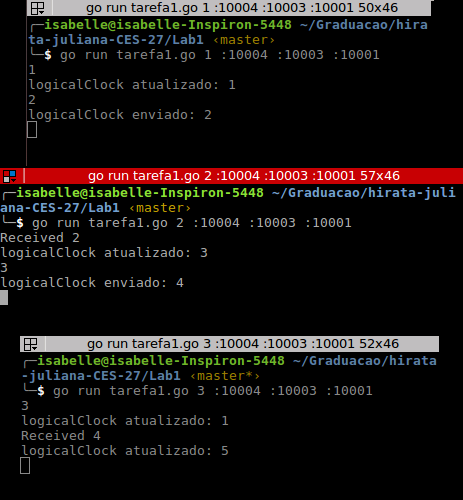
\includegraphics[scale=0.5]{imagens/tarefa1-testeslide.png}}
\caption{Sumário do modelo implementado em Keras.}.
\label{summary}
\end{figure}

	Já a Figura \ref{train/15} representa as recompensas acumulativas advindas do treinamento do modelo em 300 episódios. Esse resultado dependem diretamente da correta implementação e funcionamento dos métodos make\underline{\space}model() e act().
	
	Pode-se dizer que esse gráfico condiz com o esperado, uma vez que é possível notar inicialmente recompensas pequenas para os primeiros episódios e, mais ou menos a partir do episódio 80, tornou-se frequente recompensas com valores elevados, chegando a valores próximos de 40, indicando um aprendizado significantemente correto.

\begin{figure}[htbp]
\centering
\centerline{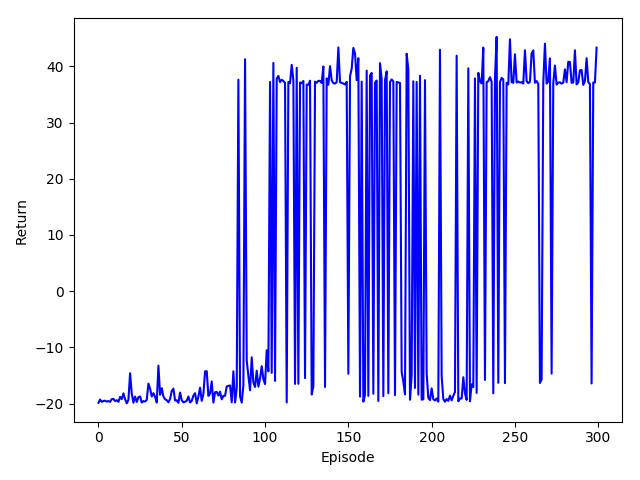
\includegraphics[scale=0.3]{imagens/train/15.png}}
\caption{Recompensa acumulativa com o passar dos episódios, no treinamento do modelo para 300 episódios.}.
\label{train/15}
\end{figure} 

	Já a aplicação do modelo implementado no ambiente do Mountain Car gerou as Figuras de \ref{dqn_evaluation} a \ref{agent_decision}.
	
	A partir da Figura \ref{dqn_evaluation}, pode-se concluir que a implementação e treino chegaram em resultados satisfatórios, uma vez que grande parte das recompensas acumuladas foi alta, próximas de 40, chegando no final de 30 episódios a uma média de 27.8, conforme apresentado na Figura \ref{evaluate_dqn_result}.
	
\begin{figure}[htbp]
\centering
\centerline{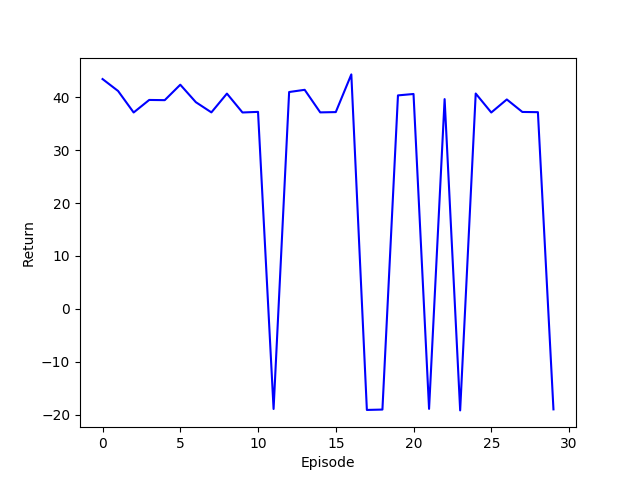
\includegraphics[scale=0.5]{imagens/dqn_evaluation.png}}
\caption{Representação em cores da tabela de action-value calculada, para algoritmo de Sarsa.}.
\label{dqn_evaluation}
\end{figure}

\begin{figure}[htbp]
\centering
\centerline{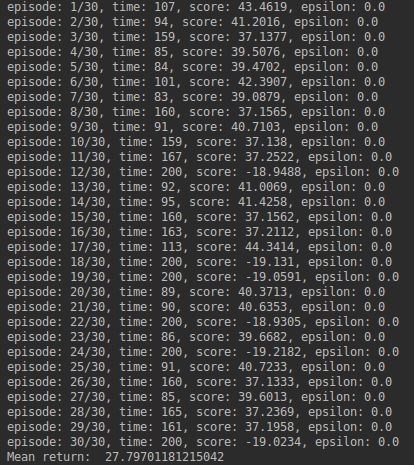
\includegraphics[scale=0.4]{imagens/evaluate_dqn_result.png}}
\caption{Recompensa acumulada em função das iterações, para algoritmo de Sarsa.}.
\label{evaluate_dqn_result}
\end{figure}
	
	Por fim, acerca da Figura \ref{agent_decision}, pode-se observar que:
	
\begin{itemize}

\item Para velocidades para direita, quase unanimamente a decisão do carro é continuar para direita. Exclui-se disso as situações de posição muito à esquerda e velocidades altas, na qual é decidido fazer nada, e de velocidades para direita muito baixas, na qual pouquíssimas vezes o carro decide ir para esquerda, talvez já se enquadrando nas intenções descritas no próximo item.

\item Para velocidades para esquerda, as decisões do carro diferem bastante da posição na qual ele se encontra. Para posições mais a esquerda, o carro decide continuar indo para esquerda, talvez para pegar impulso da subida e, quando por fim chegar em posições mais a esquerda (consequentemente mais altas) possíveis, decidir ir com velocidade para direita. Já para posições relativamente próximas da posição objetivo, aparecem também decisões de não fazer nada, indicando que o carro irá mais para esquerda e cairá na situação anteriormente descrita, na qual ele decidirá continuar indo para esquerda e pegará o impulso da elevação.

\end{itemize}

\begin{figure}[htbp]
\centering
\centerline{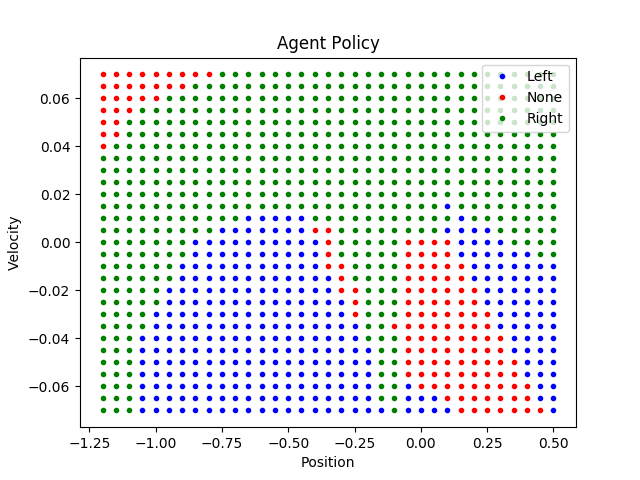
\includegraphics[scale=0.5]{imagens/agent_decision.png}}
\caption{Representação em cores da tabela de greedy-policy calculada, para algoritmo de Sarsa.}.
\label{agent_decision}
\end{figure} 

Como as decisões aprendidas e tomadas pelo carro fizeram sentido e puderam ser interpretadas satisfatoriamente, pode-se dizer que a proposta do laboratório foi corretamente implementada e se mostrou satisfatória em resolver o problema proposto.
	
\begin{thebibliography}{00}
\bibitem{roteiro} M. Maximo, ``Roteiro: Laboratório 12 - Deep Q-Learning''. Instituto Tecnológico de Aeronáutica, Departamento de Computação. CT-213, 2019.

\bibitem{roteiro8} M. Maximo, ``Roteiro: Laboratório 8 - Imitation Learning com Keras''. Instituto Tecnológico de Aeronáutica, Departamento de Computação. CT-213, 2019.

\bibitem{roteiro12} M. Maximo, ``Roteiro: Laboratório 12 - Aprendizado por Reforço Livre de Modelo''. Instituto Tecnológico de Aeronáutica, Departamento de Computação. CT-213, 2019.

\end{thebibliography}

\end{document}
